% Options for packages loaded elsewhere
\PassOptionsToPackage{unicode}{hyperref}
\PassOptionsToPackage{hyphens}{url}
%
\documentclass[
]{article}
\usepackage{amsmath,amssymb}
\usepackage{iftex}
\ifPDFTeX
  \usepackage[T1]{fontenc}
  \usepackage[utf8]{inputenc}
  \usepackage{textcomp} % provide euro and other symbols
\else % if luatex or xetex
  \usepackage{unicode-math} % this also loads fontspec
  \defaultfontfeatures{Scale=MatchLowercase}
  \defaultfontfeatures[\rmfamily]{Ligatures=TeX,Scale=1}
\fi
\usepackage{lmodern}
\ifPDFTeX\else
  % xetex/luatex font selection
\fi
% Use upquote if available, for straight quotes in verbatim environments
\IfFileExists{upquote.sty}{\usepackage{upquote}}{}
\IfFileExists{microtype.sty}{% use microtype if available
  \usepackage[]{microtype}
  \UseMicrotypeSet[protrusion]{basicmath} % disable protrusion for tt fonts
}{}
\makeatletter
\@ifundefined{KOMAClassName}{% if non-KOMA class
  \IfFileExists{parskip.sty}{%
    \usepackage{parskip}
  }{% else
    \setlength{\parindent}{0pt}
    \setlength{\parskip}{6pt plus 2pt minus 1pt}}
}{% if KOMA class
  \KOMAoptions{parskip=half}}
\makeatother
\usepackage{xcolor}
\usepackage[margin=1in]{geometry}
\usepackage{graphicx}
\makeatletter
\def\maxwidth{\ifdim\Gin@nat@width>\linewidth\linewidth\else\Gin@nat@width\fi}
\def\maxheight{\ifdim\Gin@nat@height>\textheight\textheight\else\Gin@nat@height\fi}
\makeatother
% Scale images if necessary, so that they will not overflow the page
% margins by default, and it is still possible to overwrite the defaults
% using explicit options in \includegraphics[width, height, ...]{}
\setkeys{Gin}{width=\maxwidth,height=\maxheight,keepaspectratio}
% Set default figure placement to htbp
\makeatletter
\def\fps@figure{htbp}
\makeatother
\setlength{\emergencystretch}{3em} % prevent overfull lines
\providecommand{\tightlist}{%
  \setlength{\itemsep}{0pt}\setlength{\parskip}{0pt}}
\setcounter{secnumdepth}{-\maxdimen} % remove section numbering
\usepackage{booktabs}
\usepackage{longtable}
\usepackage{array}
\usepackage{multirow}
\usepackage{wrapfig}
\usepackage{float}
\usepackage{colortbl}
\usepackage{pdflscape}
\usepackage{tabu}
\usepackage{threeparttable}
\usepackage{threeparttablex}
\usepackage[normalem]{ulem}
\usepackage{makecell}
\usepackage{xcolor}
\ifLuaTeX
  \usepackage{selnolig}  % disable illegal ligatures
\fi
\IfFileExists{bookmark.sty}{\usepackage{bookmark}}{\usepackage{hyperref}}
\IfFileExists{xurl.sty}{\usepackage{xurl}}{} % add URL line breaks if available
\urlstyle{same}
\hypersetup{
  pdftitle={Relatório Trimestral da PNAD},
  pdfauthor={Made USP},
  hidelinks,
  pdfcreator={LaTeX via pandoc}}

\title{Relatório Trimestral da PNAD\footnote{Este relatório foi
  elaborado pelas pesquisadoras do Made Eslen Brito, Clara Brenck,
  Tainari Taioka e Marina Sanches e os pesquisadores José Bergamin e
  Hiaman Santos.}}
\usepackage{etoolbox}
\makeatletter
\providecommand{\subtitle}[1]{% add subtitle to \maketitle
  \apptocmd{\@title}{\par {\large #1 \par}}{}{}
}
\makeatother
\subtitle{4º Trimestre de 2023}
\author{Made USP}
\date{20/02/2024}

\begin{document}
\maketitle

\hypertarget{a-pesquisa-nacional-por-amostra-de-domicuxedlios-contuxednua-pnad-contuxednua}{%
\section{A Pesquisa Nacional por Amostra de Domicílios Contínua (PNAD
Contínua)}\label{a-pesquisa-nacional-por-amostra-de-domicuxedlios-contuxednua-pnad-contuxednua}}

A PNAD Contínua, realizada pelo Instituto Brasileiro de Geografia e
Estatística (IBGE), é, atualmente, a principal pesquisa domiciliar
brasileira, com periodicidade trimestral e realizada de forma contínua
ao longo do ano. A PNAD Contínua é conduzida para produzir indicadores
trimestrais sobre a população brasileira, incluindo características
socioeconômicas e demográficas. Suas informações são cruciais para a
formulação e avaliação de políticas públicas e seus resultados são
amplamente utilizados por governos e pesquisadores, bem como pelo Made
em suas pesquisas.

Reportamos nossas estatísticas com recortes a partir de várias facetas
das desigualdades no Brasil: de gênero, de raça e regionais. As
variáveis de gênero e de raça são informações autodeclaradas pela(o)
entrevistada(o). Nós utilizamos duas categorias de raça: negros (que
considera pretos e pardos) e brancos.

Reportamos as estatísticas comparativamente ao mesmo trimestre de 2022,
bem como ao trimestre anterior (3º trimestre de 2023). Este relatório
pretende ser informativo e, portanto, não busca discutir os motivos por
trás de possíveis mudanças nos indicadores. O acesso às estatísticas e
tabelas completas pode ser feito por meio de links disponibilizados no
final do documento.

A PNAD Contínua divulgada em 16/02/2024 apresenta dados referentes ao 4º
trimestre de 2023 - de setembro a dezembro.

\hypertarget{mercado-de-trabalho}{%
\section{Mercado de Trabalho}\label{mercado-de-trabalho}}

\hypertarget{taxa-de-participauxe7uxe3o}{%
\subsection{Taxa de Participação}\label{taxa-de-participauxe7uxe3o}}

A taxa de participação refere-se ao percentual da população em idade de
trabalhar que participa da força de trabalho\footnote{A metodologia de
  cálculo desta taxa exclui da força de trabalho os que não procuram
  emprego nem estão trabalhando, como aposentados, donas de casa e
  estudantes.}. No 4º trimestre de 2023, a taxa de participação no
mercado de trabalho de homens negros foi de 72.36\% e a de homens
brancos, 72.33\%. A taxa de participação no mercado de trabalho ficou em
54.15\% para mulheres brancas e 51.64\% para mulheres negras.

Em comparação com o trimestre anterior (3º trimestre de 2023), houve
pouca variação na taxa de participação destes grupos. Isso também é
verdade em relação ao mesmo trimestre do ano anterior (4º trimestre de
2022), em que a registraram-se taxas de participação de 51.6\% e
54.13\%, para mulheres negras e brancas, respectivamente; e de cerca de
72\% para homens brancos e negros.

Em relação às desigualdades regionais, percebemos grande variação na
taxa de participação no mercado de trabalho por região do país. A região
Nordeste é aquela que tem menor taxa de participação no mercado de
trabalho, ficando em 54.21\%, na média. Na região Nordeste, todos os
grupos demográficos têm menor taxa de participação do que nas demais
regiões. As regiões Centro-Oeste e Sul são as que apresentam maior taxa
de participação no mercado de trabalho, de 67.77\% e 66.08\%,
respectivamente. Tais valores também se mantiveram estáveis quando
comparados ao 3º trimestre de 2023 e ao 4º trimestre de 2022.

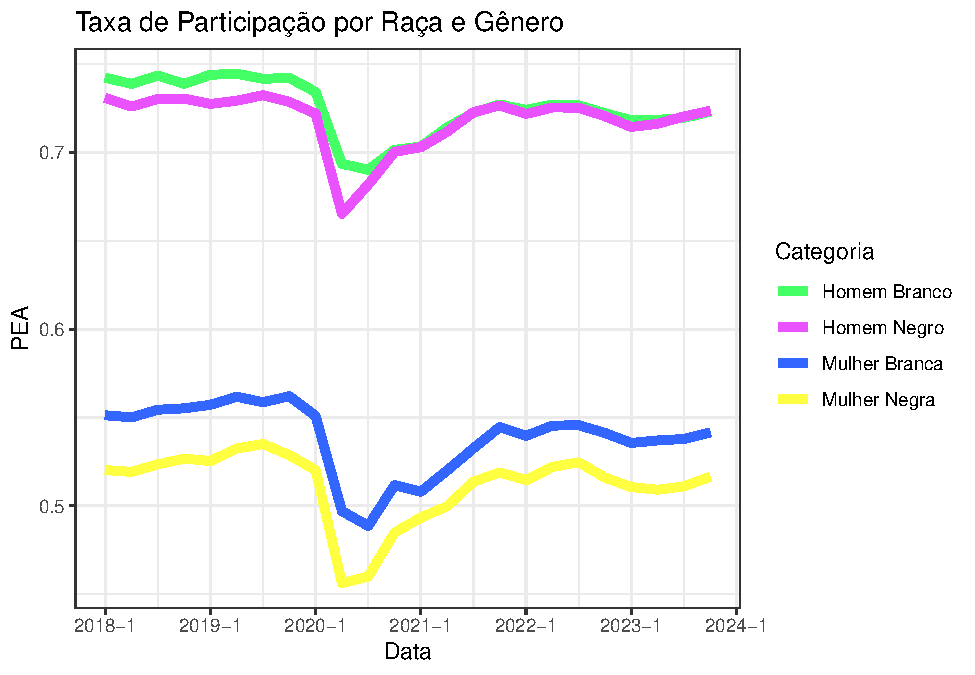
\includegraphics{R-Markdown--Long-Version-_files/figure-latex/unnamed-chunk-5-1.pdf}

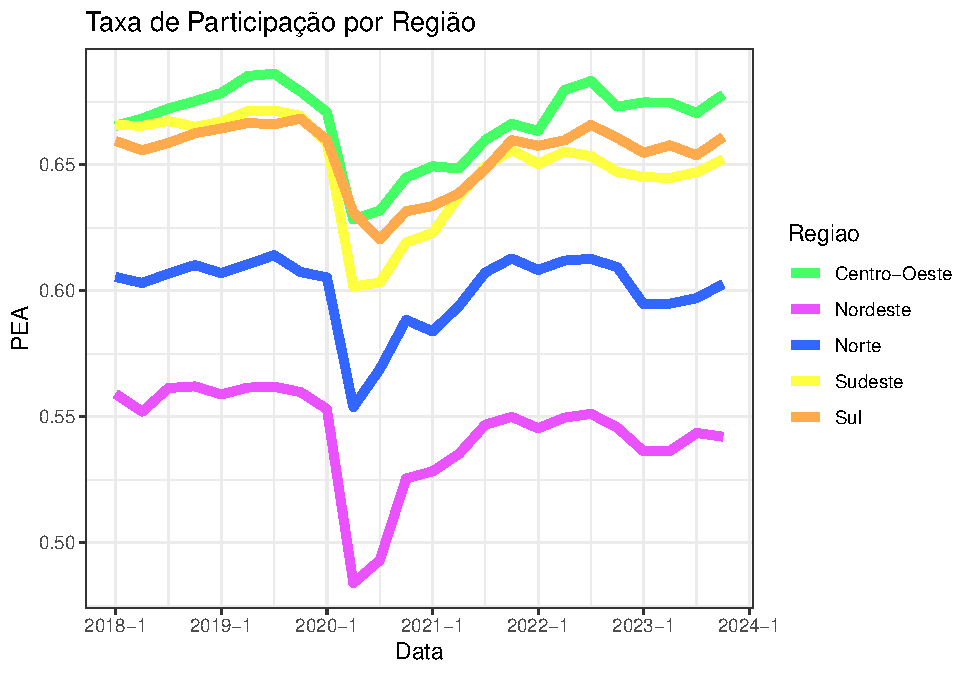
\includegraphics{R-Markdown--Long-Version-_files/figure-latex/unnamed-chunk-7-1.pdf}

\hypertarget{emprego-desemprego-e-escolaridade}{%
\subsection{Emprego, desemprego e
escolaridade}\label{emprego-desemprego-e-escolaridade}}

\hypertarget{ocupauxe7uxe3o}{%
\subsubsection{Ocupação}\label{ocupauxe7uxe3o}}

No 4º trimestre de 2023, o desemprego ficou em 7.41\% no Brasil, uma
queda de -0.28 pontos percentuais em relação ao trimestre anterior. O
desemprego no país no 4º trimestre de 2022 tinha atingido 8.7\%. Houve,
portanto, uma importante queda deste indicador no período de um ano. A
categoria de Homem Branco foi quem teve a maior taxa de emprego,
enquanto a de Mulher Negra foi quem teve a menor.

Observamos que a taxa de desemprego das mulheres negras foi de \% e,
para as mulheres brancas, o desemprego ficou em \%. Os homens brancos
tiveram taxa de desemprego no patamar de \%. Para os homens negros, a
taxa foi de \%.

No período de um ano, isto é, comparando-se os dados do trimestre de
referência com o mesmo período de 2022, a situação melhorou. O
desemprego entre homens brancos caiu pontos percentuais e, o de homens
negros, p.p. Para as mulheres brancas, o desemprego teve um recuo de
p.p. e, para mulheres negras, registrou-se queda de pontos percentuais.

Regionalmente, o desemprego também apresentou tendência de queda no 4º
trimestre de 2023. A região Norte, registrou a maior taxa de desemprego
de 10.44\% (queda de -0.35 pontos percentuais em um ano). A menor taxa
de desemprego foi registrada na região Sul, 4.5\%, com diferença de 0.03
p.p. em um ano. Na região Nordeste, a taxa de desemprego registrada foi
de 10.44\% (recuo de -0.42 p.p. em um ano). Na região Centro-Oeste, a
taxa de desemprego medida foi de 5.76\% (queda de -0.43 p.p. em um ano).
Por fim, na região Sudeste, a taxa de desemprego registrada foi de 7.1\%
(recuo de -0.81 p.p. em um ano).

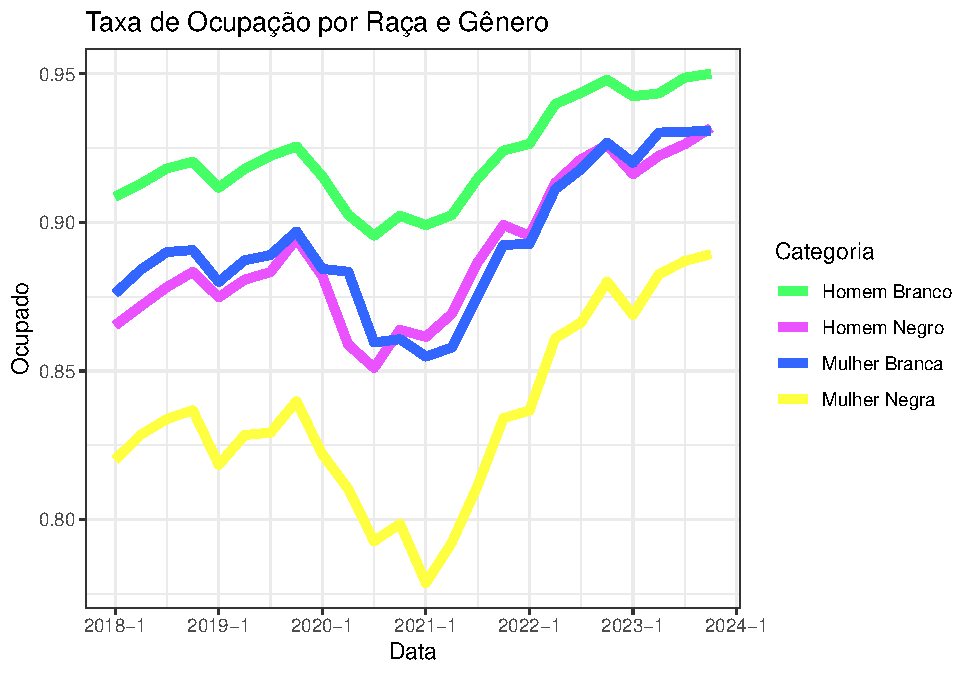
\includegraphics{R-Markdown--Long-Version-_files/figure-latex/unnamed-chunk-10-1.pdf}

\hypertarget{escolaridade}{%
\subsubsection{Escolaridade}\label{escolaridade}}

Dados de escolaridade representam o percentual de obtenção de um grau
educacional dentro de um designado grupo da população economicamente
ativa. Dentre as mulheres negras, 18.01\% possíam ensino superior,
52.56\%, ensino médio e, 23.39\%, apenas ensino fundamental. Para as
mulheres brancas, 30.57\% tinham ensino superior completo, 40.66\%,
ensino médio e 15.43\%, ensino fundamental.

Dentre os homens negros, 11.89\% haviam obtido ensino superior, 50.53\%,
ensino médio e 33.58\%, ensino fundamental. Dos homens brancos, 23.46\%
tinham ensino superior, 44.05\% ensino médio e 23.65\%, apenas ensino
fundamental.

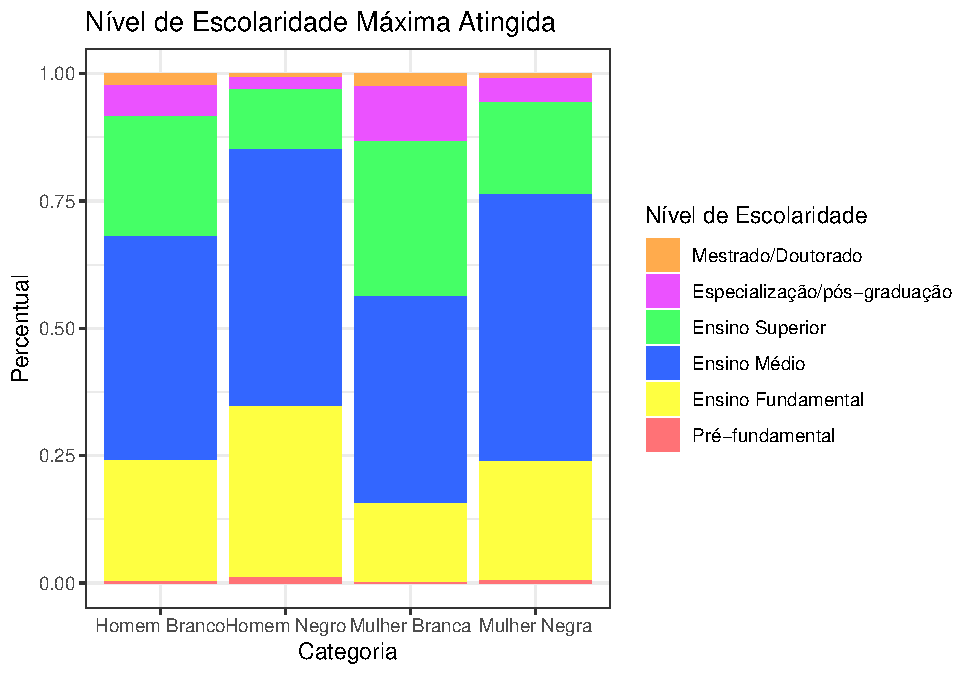
\includegraphics{R-Markdown--Long-Version-_files/figure-latex/unnamed-chunk-12-1.pdf}

\hypertarget{formalidade-e-informalidade}{%
\subsubsection{Formalidade e
Informalidade}\label{formalidade-e-informalidade}}

No Brasil, tradicionalmente adota-se a falta de carteira assinada como
critério para a definição de informalidade do trabalho. Outro critério,
bem estabelecido na literatura e utilizado neste relatório, considera a
não contribuição à seguridade social para a caracterização da
informalidade\footnote{Ver Kassouf, A. L. Wage gender discrimination and
  segmentation in the Brazilian labor market. Economia Aplicada, v. 2,
  n.~2, p.~243-269, 1998. Disponível em: Vista do Wage gender
  discrimination and segmentation in the Brazilian labor market
  (usp.br). Acesso em: 16/11/2023; e Dalberto, C. e Cirino, J.
  Informalidade e segmentação no mercado de trabalho brasileiro:
  evidências quantílicas sob alocação endógena. Nova Economia. v.28 n.2
  p.417-460, 2018. Disponível em:
  \url{https://doi.org/10.1590/0103-6351/3191}. Acesso em 16/11/2023.}.
Esse critério é útil para a captura dos trabalhadores autônomos e
empregados informais nas pesquisas, sobretudo ao levar-se em conta a
questão da precariedade do trabalho. Sem amparo do sistema de seguridade
social, tais trabalhadores encontram-se, portanto, em posição mais
vulnerável. Benefícios relacionados à proteção da renda em caso de
doença, velhice ou maternidade, por exemplo, não são recebidos por tais
trabalhadores.

Neste sentido, consideramos a porcentagem de trabalhadores que
contribuem para o instituto de previdência (indicado por ``contribuinte
INSS'') e o percentual daqueles que não contribuem -- que se encontram,
portanto, em situação de informalidade. Reportamos que 29.22, 29.52,
29.72, 29.95, 29.72, 30.54, 30.94, 30.31, 29.17, 27.72, 28.57, 29.19,
29.42, 30.11, 30.75, 30.92, 30.36, 30.47, 30.49, 28.65, 29.84, 29.61,
29.55, 29.53\% dos trabalhadores brancos e 43.12, 43.1, 43.82, 43.36,
43.32, 43.57, 44.1, 43.48, 43.57, 40.88, 42.83, 43.27, 43.1, 44.23,
44.39, 44.21, 43.95, 43.37, 42.81, 42.15, 42.16, 42.06, 42.13, 41.54\%
dos trabalhadores negros estavam na informalidade no 4º trimestre de
2023. Entre as mulheres, 27.74, 28.09, 28.35, 28.38, 27.98, 28.78,
29.31, 29.02, 28.47, 25.77, 25.68, 26.4, 26.21, 27.71, 28.84, 29.54,
28.76, 28.9, 28.33, 27.53, 26.92, 27.19, 27.7, 27.28\% das trabalhadoras
brancas e 40.99, 40.8, 41.82, 41.33, 40.6, 41.98, 42.01, 41.61, 41.1,
37.35, 38.59, 40.74, 39.38, 40.56, 41.24, 41.28, 40.91, 41.15, 40.93,
39.66, 39.08, 39.74, 39.52, 39\% das trabalhadoras negras não constavam
como contribuintes da previdência.

Percebe-se ainda que a taxa de informalidade entre as pessoas negras foi
maior do que a taxa média para todos os trabalhadores, de 35.18\%, no 4º
trimestre de 2023. Registrou-se queda de -0.13 pontos percentuais na
informalidade média da economia brasileira, em comparação com o mesmo
trimestre de 2022.

As regiões com maiores taxas de informalidade são a Norte e Nordeste,
com taxas iguais a 51.27\% e 50.72\%, respectivamente. A taxa de
informalidade da região Sul é a menor, 23.23\%, enquanto que as regiões
Sudeste e Centro-Oeste registram 29.41\% e 31.84\% de informalidade em
sua força de trabalho, respectivamente.

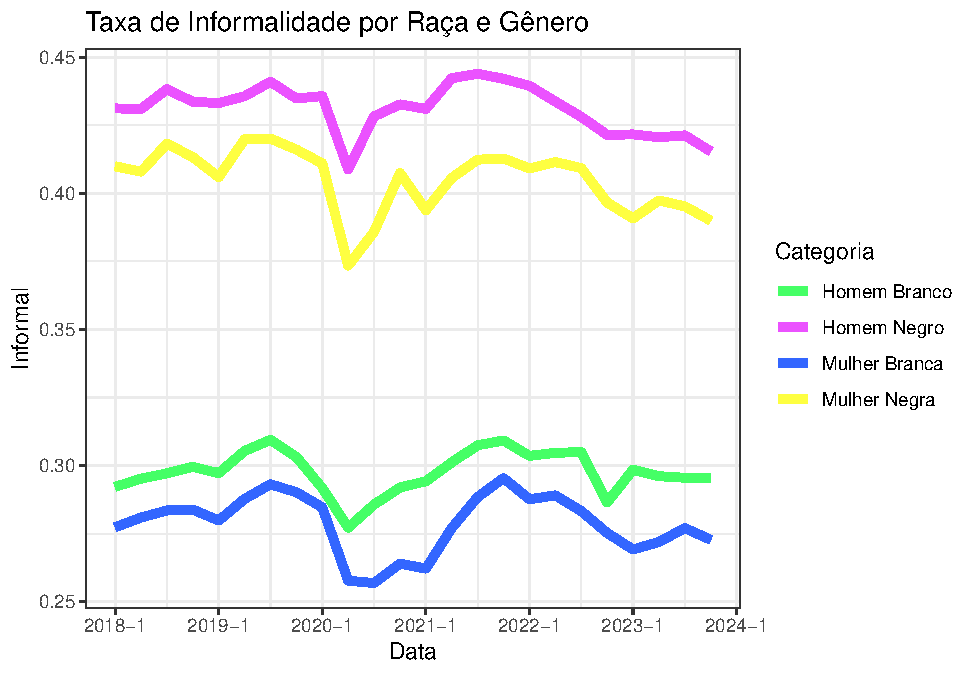
\includegraphics{R-Markdown--Long-Version-_files/figure-latex/unnamed-chunk-15-1.pdf}

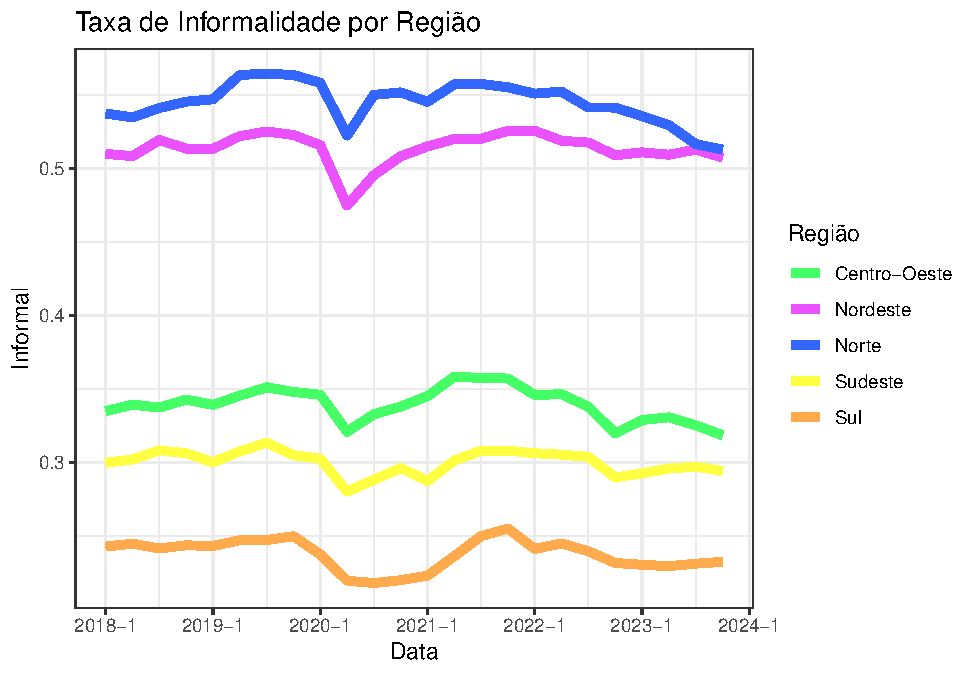
\includegraphics{R-Markdown--Long-Version-_files/figure-latex/unnamed-chunk-17-1.pdf}

\hypertarget{subocupauxe7uxe3o}{%
\subsubsection{Subocupação}\label{subocupauxe7uxe3o}}

Reportamos as estatísticas de subocupação no mercado de trabalho. O
intuito desse indicador é complementar o monitoramento do mercado de
trabalho, para além da taxa de desocupação. Ela capta três informações
principais, são elas: i) trabalhou habitualmente menos de 40 horas no
seu único trabalho ou no conjunto de todos os seus trabalhos, ii)
preferia trabalhar mais horas do que as habitualmente trabalhadas e,
iii) estava disponível para trabalhar mais horas no período de 30 dias,
contados a partir do primeiro dia da semana de referência.

No 4º trimestre de 2023, a taxa de subocupação foi de 3.32\% para os
homens brancos e 5.51\% para os homens negros. Já para as mulheres, tal
taxa foi de 4.79\% para as trabalhadoras brancas e 7.9\% para as negras.

A região Nordeste foi a que apresentou maior taxa média se subocupação,
de 10.21\%, seguida pela região Centro-Oeste (3.36\%), Sudeste (4.14\%),
Norte (5.95\%) e, por último, a região Sul, com 2.91\% dos trabalhadores
subocupados.

\hypertarget{emprego-por-setor}{%
\subsection{Emprego por setor}\label{emprego-por-setor}}

A ocupação por setores no Brasil também varia consideravelmente de
acordo com a raça e o gênero. No 4º trimestre de 2023, a maioria dos
homens negros (NA\%) estava alocada no setor de comércio. Seguem-se os
setores de construção e de indústria, com NA\% e NA\% da alocação da
força de trabalho de homens negros, respectivamente. Para homens
brancos, o setor que mais emprega também é o comércio NA\%), além da
indústria, com NA\%, setor de informação, que emprega NA\%, e
agricultura, com NA\%.

Para o total de mulheres brancas empregadas, NA\% estão no setor de
educação, NA\% encontram-se no setor de comércio e NA\% no setor de
informação. Das mulheres negras, NA\% estão alocadas no setor de
educação, seguido do comércio, NA\%, e serviços domésticos, com NA\%.
Nota-se que o setor de informação emprega mais brancos que negros e os
serviços domésticos são majoritariamente exercidos por mulheres negras.

As composições em relação a gênero e raça dos setores para as diferentes
regiões brasileiras apresentam algumas particularidades. Para as
mulheres, os empregos setoriais são bem parecidos com os resultados
gerais. Já no caso dos homens, há diferenças entre as regiões. Por
exemplo, no Nordeste e no Centro-Oeste, a maioria dos homens (brancos e
negros) estão no setor de agricultura, enquanto que no Sudeste e Norte,
a maior parte deles encontra-se no setor de comércio. No Sul, o setor
que mais emprega os homens é a indústria.

\hypertarget{rendimento}{%
\section{Rendimento}\label{rendimento}}

\hypertarget{rendimento-efetivo-e-habitual}{%
\subsection{Rendimento Efetivo e
Habitual}\label{rendimento-efetivo-e-habitual}}

Nesta seção apresentamos os rendimentos mensais dos trabalhadores em seu
trabalho principal com recorte de raça e gênero. Os rendimentos são
reportados em termos reais, isto é, deflacionados e a preços do ano de
2023.

O rendimento habitual mensal do trabalho principal consiste no
rendimento recebido pelo trabalhador sem considerar acréscimos e
descontos esporádicos. Já o rendimento efetivo mensal do trabalho
principal inclui os pagamentos e descontos que não possuem caráter
contínuo.

Os dados apontam que o rendimento habitual médio do trabalhador
brasileiro foi de R\$ 2946.54 por mês no 4º trimestre de 2023. Para
mulheres e homens brancos, foram registrados rendimentos habituais acima
da média: de R\$ 3246.5/mês, para mulheres brancas; e de R\$
4229.79/mês, para homens brancos. A renda habitual foi menor do que a
média para os negros: de R\$ 1957.36/mês, para mulheres negras; e de R\$
2466.76/mês, para homens negros.

Na média, o rendimento efetivo do brasileiro foi de R\$ 3050.42 mensais
no 4º trimestre de 2023. Novamente, operam desigualdades de raça e
gênero. Para mulheres brancas e homens brancos, registraram-se
rendimentos efetivos de R\$ 3370.74/mês e R\$ 4376.15/mês,
respectivamente. Para mulheres negras e homens negros, o rendimento
efetivo foi de R\$ 2035.94/mês e R\$ 2545.6/mês, respectivamente.

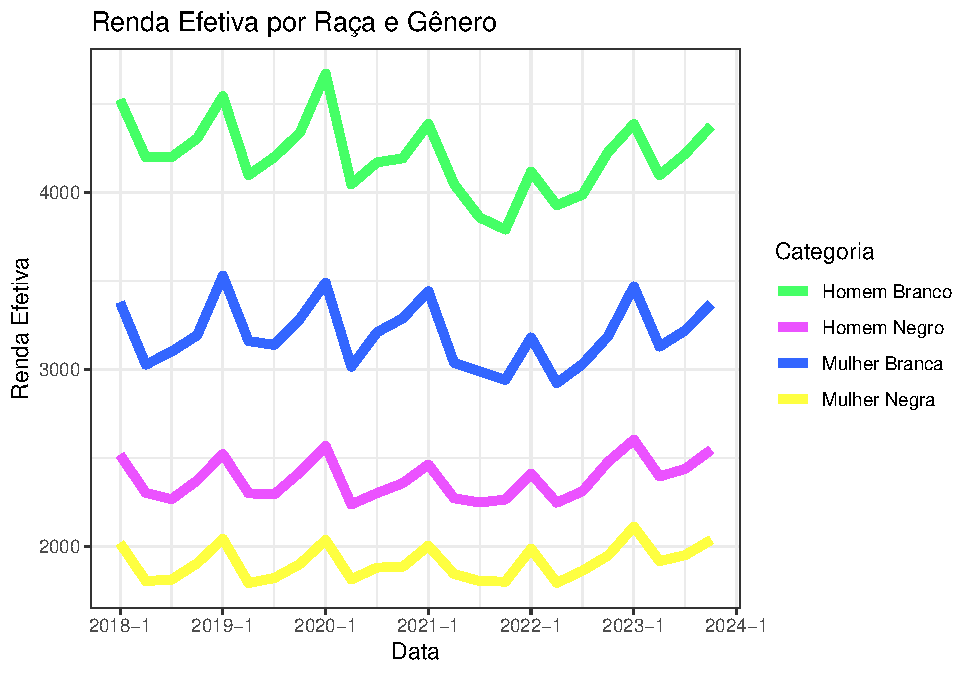
\includegraphics{R-Markdown--Long-Version-_files/figure-latex/unnamed-chunk-21-1.pdf}

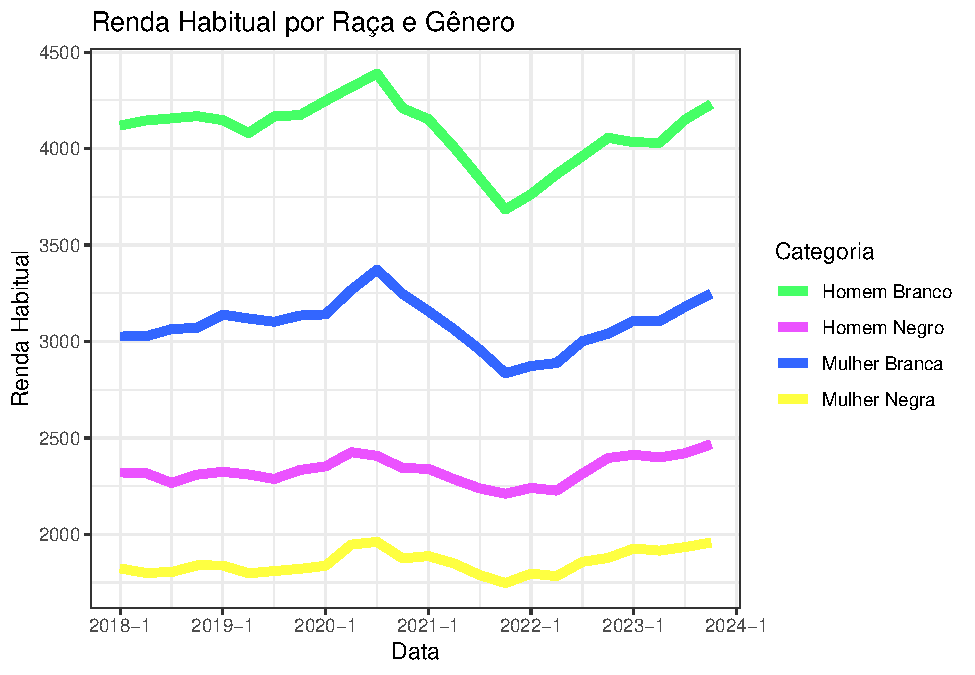
\includegraphics{R-Markdown--Long-Version-_files/figure-latex/unnamed-chunk-23-1.pdf}

\hypertarget{distribuiuxe7uxe3o-gini}{%
\subsection{Distribuição: Gini}\label{distribuiuxe7uxe3o-gini}}

O índice de Gini varia de zero a um, sendo que quanto mais próximo de
um, maior a desigualdade. Por exemplo, em uma situação hipotética em que
o índice de Gini é igual a zero, todos os indivíduos de uma determinada
sociedade possuem a mesma renda (igualdade). Já a outra situação
hipotética extrema, com um índice igual a um, indica que somente uma
pessoa detém toda a renda dessa economia\footnote{Para o cálculo do
  índice de Gini, consideramos a renda que os trabalhadores efetivamente
  receberam, isto é, seu rendimento efetivo em todos os trabalhos.}.

O índice de Gini dos rendimentos efetivos a nível nacional para o 4º
trimestre de 2023 foi de 0.51. Esse índice não se alterou
comparativamente ao trimestre anterior e ao 4º trimestre de 2022,
indicando uma estabilidade do nível de desigualdade dos rendimentos no
último ano\footnote{Por tratar-se de pesquisa amostral, a PNADc tem
  limitações na captura de rendas dos mais ricos, sobretudo rendimentos
  de capital. Ademais, a literatura documenta a existência de
  subnotificação de rendas provenientes de transferências
  governamentais, já que a PNAD não se pretende representativa apenas de
  quem recebe transferências de renda, conforme Souza, Osorio, \& Soares
  2011; e Souza,Osorio, Paiva, et al.~2019.}.

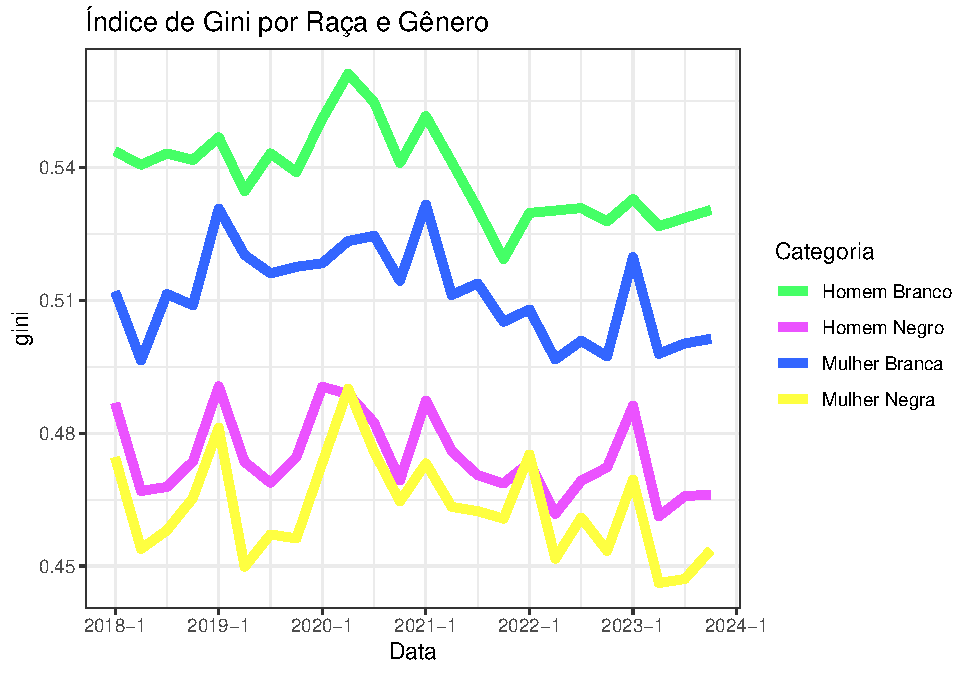
\includegraphics{R-Markdown--Long-Version-_files/figure-latex/unnamed-chunk-25-1.pdf}

\includegraphics{R-Markdown--Long-Version-_files/figure-latex/unnamed-chunk-27-1.pdf}

Observamos que as regiões Nordeste e Norte apresentam desigualdade
levemente maior do que a reportada para todo o território nacional no
trimestre analisado, com índices de Gini iguais a e , respectivamente.
Para as outras regiões, calcularam-se os seguintes índices de Gini:
Centro-Oeste, ; Sudeste, ; e Sul, .

Em relação ao recorte de raça e gênero, calcularam-se os seguintes
índices de Gini: para os homens brancos, ; para os homens negros, ; para
as mulheres brancas, ; e, para as mulheres negras, .

\hypertarget{percentis-de-renda}{%
\subsection{Percentis de renda}\label{percentis-de-renda}}

Outra forma de estudarmos a desigualdade de rendimentos, além do cálculo
do Índice de Gini, é analisando os percentis de renda. Os percentis,
decis e quantis são calculados ordenando a população de forma crescente
a partir do nível de renda. Se uma economia possui 100 pessoas, por
exemplo, ordenam-se essas pessoas por ordem de renda e divide-se a
população em grupos com o mesmo número de pessoas. Se desejamos os
quantis dessa economia, dividimos essas 100 pessoas em quatro grupos,
cada grupo de tamanho igual, isto é, com 25 pessoas. Dito de outra
maneira, para obter os quantis, a população é dividida em partes de 25\%
cada. Por exemplo: Q1 representa a renda que separa os 25\% da população
com menor renda dos demais, Q2 corresponde à renda que separa os 50\%
mais pobres e Q3 corresponde aos 75\% mais pobres.

\begin{figure}
\centering
\includegraphics[width=0.9\textwidth,height=\textheight]{C:/Users/clara/Downloads/quantis_exemplo.png}
\caption{Separação de Dados em Quantis: Exemplo}
\end{figure}

Além disso, os quantis podem ser subdivididos em mais segmentos, como é
o caso dos decis, em que se divide a população em 10 grupos -- cada
grupo contendo 10\% da população. Por fim, os dados ainda podem ser
subdivididos em percentis, neste caso a população é dividida em
centésimas partes, cada parte teria 1\% dos dados.

Para calcular uma medida de distribuição de renda, obtemos a renda
apropriada por cada um dos decis da distribuição de renda, juntamente
com o último percentil, que é o valor equivalente ao 1\% mais rico da
população. Assim, encontramos o percentual da renda total do país que
está nas mãos das pessoas em cada grupo de renda específico. Reportamos
a participação de cada um dos quantis de renda na renda total do país.
Por exemplo, o último percentil (ou o 1\% mais rico) apropriou-se de X\%
da renda nacional, no terceiro trimestre de 2023. Esse número é x\%
maior/ menor que sua participação no trimestre do ano anterior.

A partir desses dados, podemos construir uma curva de Lorenz para o
Brasil para o terceiro trimestre de 2023. Para construir a curva de
Lorenz, acumulamos os dados reportados acima, da população e da renda: a
curva mostra como a proporção da renda total aumenta em função da
proporção da população (Hoffmann, 1998).

Na situação hipotética de total igualdade em que todas as pessoas
possuem o mesmo rendimento efetivo, a curva de Lorenz da economia seria
o segmento de reta desenhado no gráfico, que chamamos de linha de
perfeita igualdade. Assim, quanto mais afastada dessa linha a curva de
Lorenz de um país está, maior o grau de desigualdade de rendimentos. Por
definição, o Índice de Gini é igual à razão entre: a área entre a linha
de perfeita igualdade e a curva de Lorenz, e a área total abaixo da
linha de perfeita igualdade\footnote{ver Hoffmann, 1998.}.

\includegraphics{R-Markdown--Long-Version-_files/figure-latex/unnamed-chunk-28-1.pdf}

\includegraphics{R-Markdown--Long-Version-_files/figure-latex/unnamed-chunk-29-1.pdf}

\hypertarget{tabelas-completas}{%
\section{Tabelas completas}\label{tabelas-completas}}

Por fim, são disponibilizadas as tabelas com dados completos:

\href{https://drive.google.com/file/d/1MszWt8l3aHwKP5v78_gP-sGT0e-wqccx/view?usp=sharing}{Tabela
1: Dados por Raça e Gênero}

\href{https://drive.google.com/file/d/1bCn8967ccAvB3idm5PiwU31HIFqY680K/view?usp=sharing}{Tabela
2: Dados por Região}

\href{https://drive.google.com/file/d/10pwdVV6pGg4FgjZuXLQR6h7l1Zkplgmq/view?usp=sharing}{Tabela
3: Dados por Raça, Gênero e Região}

\href{https://drive.google.com/file/d/1qThm-hEmr9hotuPpOQu8jvqbbGNkMHBs/view?usp=sharing}{Tabela
4: Dados para a média do Brasil}

\end{document}
